\documentclass[letterpaper,12pt]{article}
\usepackage{array}
\usepackage{threeparttable}
\usepackage{geometry}
\geometry{letterpaper,tmargin=1in,bmargin=1in,lmargin=1.25in,rmargin=1.25in}
\usepackage{fancyhdr,lastpage}
\pagestyle{fancy}
\lhead{}
\chead{}
\rhead{}
\lfoot{}
\cfoot{}
\rfoot{\footnotesize\textsl{Page \thepage\ of \pageref{LastPage}}}
\renewcommand\headrulewidth{0pt}
\renewcommand\footrulewidth{0pt}
\usepackage[format=hang,font=normalsize,labelfont=bf]{caption}
\usepackage{listings}
\lstset{frame=single,
  language=Python,
  showstringspaces=false,
  columns=flexible,
  basicstyle={\small\ttfamily},
  numbers=none,
  breaklines=true,
  breakatwhitespace=true
  tabsize=3
}
\usepackage{amsmath}
\usepackage{amssymb}
\usepackage{amsthm}
\usepackage{harvard}
\usepackage{setspace}
\usepackage{float,color}
\usepackage{graphicx}
\usepackage{hyperref}
\hypersetup{colorlinks,linkcolor=red,urlcolor=blue}
\theoremstyle{definition}
\newtheorem{theorem}{Theorem}
\newtheorem{acknowledgement}[theorem]{Acknowledgement}
\newtheorem{algorithm}[theorem]{Algorithm}
\newtheorem{axiom}[theorem]{Axiom}
\newtheorem{case}[theorem]{Case}
\newtheorem{claim}[theorem]{Claim}
\newtheorem{conclusion}[theorem]{Conclusion}
\newtheorem{condition}[theorem]{Condition}
\newtheorem{conjecture}[theorem]{Conjecture}
\newtheorem{corollary}[theorem]{Corollary}
\newtheorem{criterion}[theorem]{Criterion}
\newtheorem{definition}[theorem]{Definition}
\newtheorem{derivation}{Derivation} % Number derivations on their own
\newtheorem{example}[theorem]{Example}
\newtheorem{exercise}[theorem]{Exercise}
\newtheorem{lemma}[theorem]{Lemma}
\newtheorem{notation}[theorem]{Notation}
\newtheorem{problem}[theorem]{Problem}
\newtheorem{proposition}{Proposition} % Number propositions on their own
\newtheorem{remark}[theorem]{Remark}
\newtheorem{solution}[theorem]{Solution}
\newtheorem{summary}[theorem]{Summary}
%\numberwithin{equation}{section}
\bibliographystyle{aer}



\begin{document}

\begin{flushleft}
  \textbf{\large{Problem Set 5}} \\
  MACS 40000, Dr. Evans \\
  Fiona Fan
\end{flushleft}

\vspace{5mm}

\noindent\textbf{Problem 7.3 (a)}\\
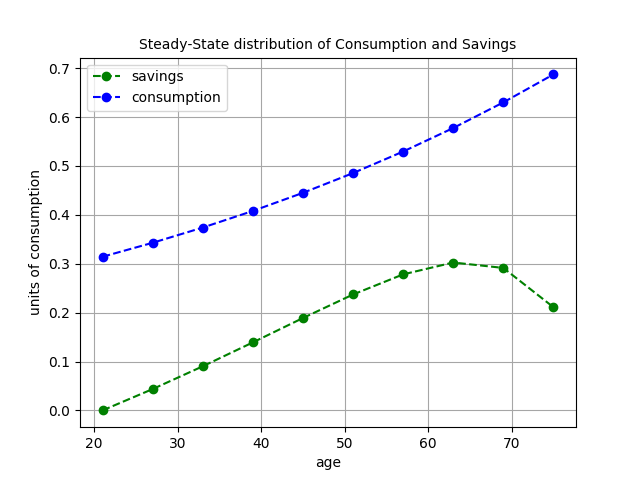
\includegraphics[scale=0.5]{images_SS/ss_bc.png}
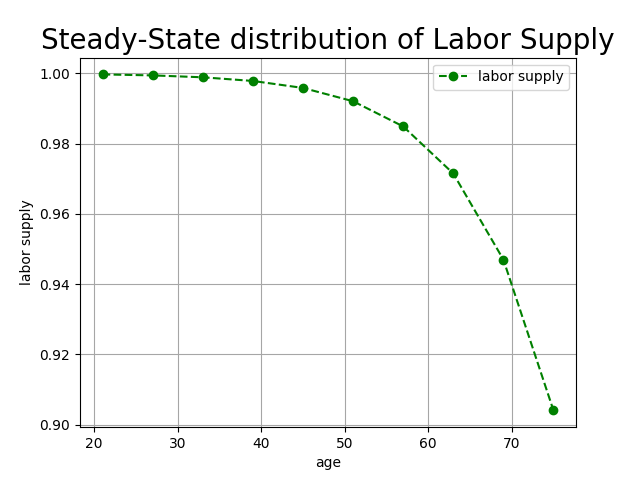
\includegraphics[scale=0.5]{images_SS/ss_n}\\
\\
\noindent\textbf{Problem 7.3 (b)}\\
\begin{table}[htbp!]\centering
\begin{tabular}{|l|c|}\hline
 $\bar{r}$ & 0.72\\
 $\bar{w}$ & 0.36\\
 $\bar{K}$ & 1.78\\
 $\bar{L}$ &9.79\\
 $\bar{Y}$ &5.39\\
 $\bar{C}$ &4.79\\
 Savings Euler Error & $3.1e^{-5}$\\
 Labor Euler Error & $5.95e^{-14}$\\
 Last period saving & $7.6e^{-5}$\\
 Resource Constraint Error & $-1.13e^{-9}$\\ \hline
\end{tabular}
\end{table}
\\
\noindent\textbf{Problem 2(a)}\\
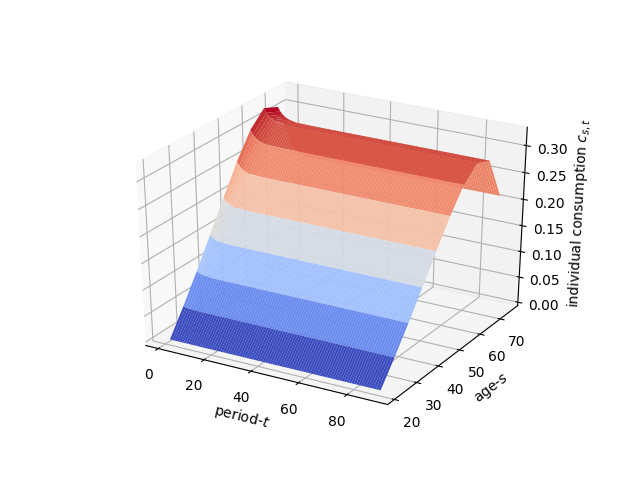
\includegraphics[scale=0.35]{images_TPI/cpath}
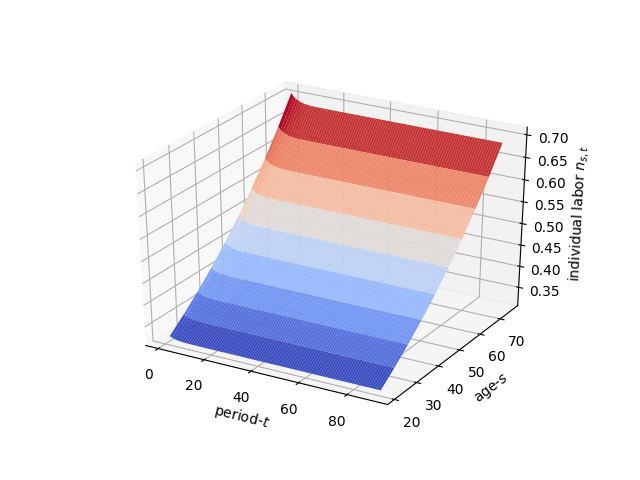
\includegraphics[scale=0.35]{images_TPI/npath}
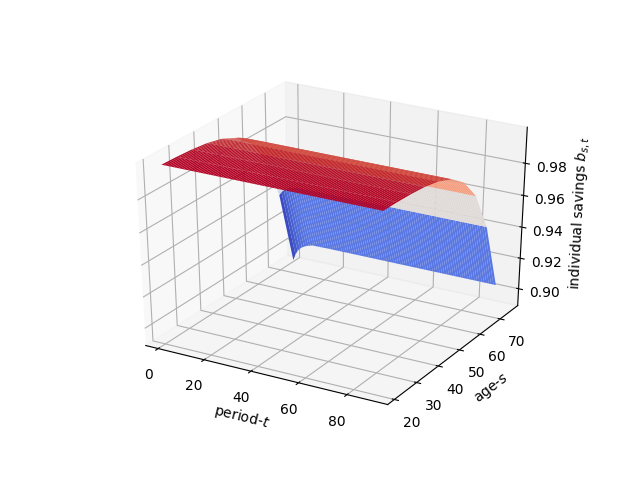
\includegraphics[scale=0.35]{images_TPI/bpath}
\\
\noindent\textbf{Problem 2(b)}\\
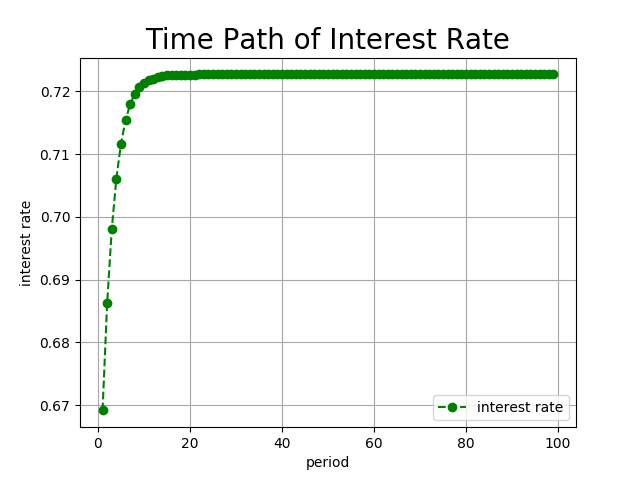
\includegraphics[scale=0.35]{images_TPI/tpi_r}
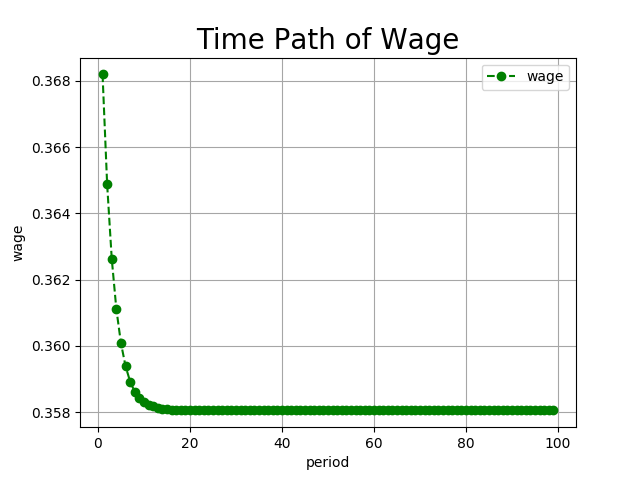
\includegraphics[scale=0.35]{images_TPI/tpi_w}
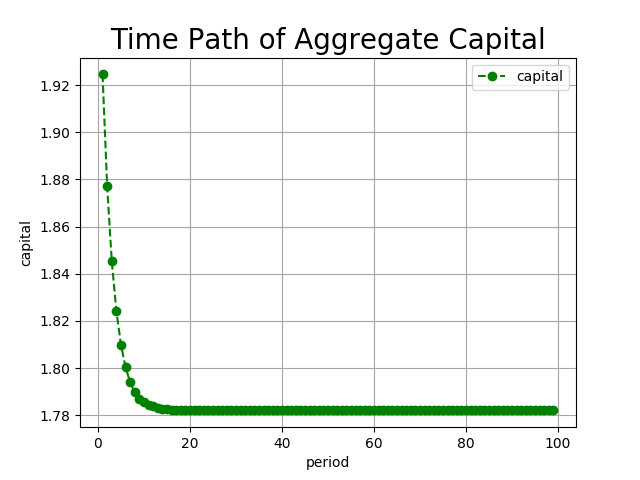
\includegraphics[scale=0.35]{images_TPI/tpi_K}
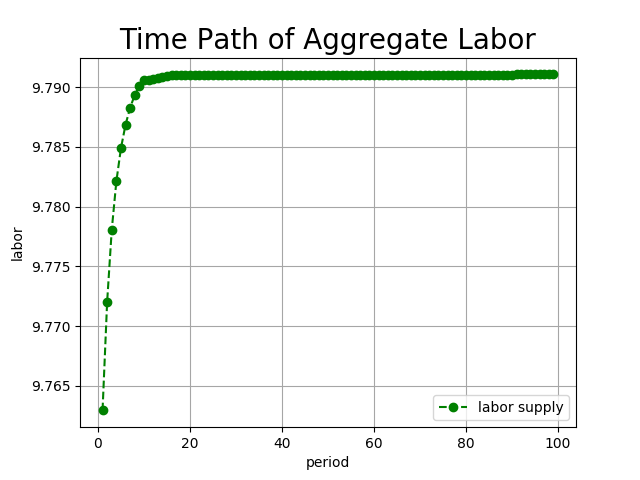
\includegraphics[scale=0.35]{images_TPI/tpi_L}
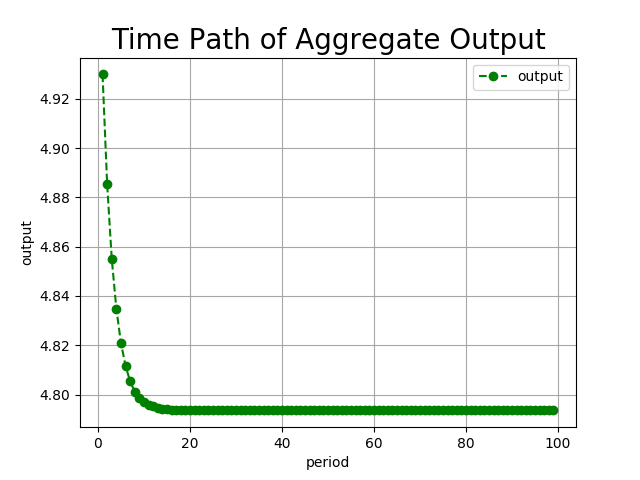
\includegraphics[scale=0.35]{images_TPI/tpi_Y}
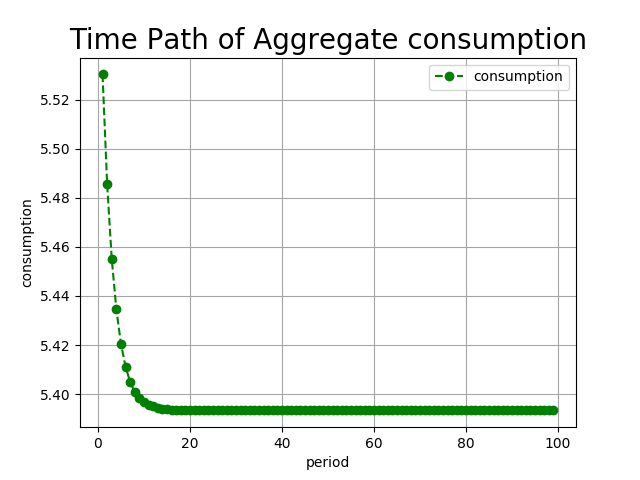
\includegraphics[scale=0.35]{images_TPI/tpi_C}
\\
\noindent\textbf{Problem 2(c)}\\
\begin{table}[htbp!]\centering
\begin{tabular}{|l|c|}\hline
 Savings Euler Error & $0.55$\\
 Labor Euler Error & $8.43e^{-6}$\\
 Last period saving & $0.23$\\
 Resource Constraint Error & $2.67e^{-5}$\\ \hline
\end{tabular}
\end{table}

\noindent\textbf{Problem 2(d)}\\
$T$ is 20 for the economy to get 0.0001 within $\bar{K}$.
\end{document}